\documentclass[svgnames,10pt]{article}
\usepackage[margin=1in]{geometry}
\usepackage[T1]{fontenc}
\usepackage{times}
\renewcommand\thesection{(\alph{section})}
\renewcommand\thesubsection{(\alph{subsection})}
\usepackage[parfill]{parskip}
\usepackage{calc}
\usepackage{amsmath}
\usepackage{amsfonts}

\usepackage{lastpage}
%\newcommand{\pageoflastpage}{Page {\thepage} of \pageref*{LastPage}}
%\newcommand{\pageoflastpage}{{\thepage} of \pageref*{LastPage}}
\newcommand{\pageoflastpage}{}
% \newcommand*{\DEBUG}{}
\ifdefined\DEBUG
\newcommand{\simone}[1]{\todo[inline,size=\small, color=green!40]{S: #1}}
\else
\newcommand{\simone}[1]{}
\fi
\newcommand{\ganesh}[1]{\todo[inline,size=\small, color=yellow!40]{G: #1}}
\newcommand{\zvonimir}[1]{\todo[inline,size=\small, color=blue!40]{Z: #1}}
\newcommand{\dong}[1]{\todo[inline,size=\small, color=red!40]{D: #1}}
\newcommand{\ignacio}[1]{\todo[inline,size=\small, color=yellow!40]{I: #1}}
\newcommand{\greg}[1]{\todo[inline,size=\small, color=yellow!40]{L: #1}}
\newcommand{\martin}[1]{\todo[inline,size=\small, color=yellow!40]{M: #1}}

\newcommand{\archer}{\textsc{Archer}\xspace}
\newcommand{\tsan}{TSan\xspace}
\newcommand{\iomp}{Intel\circledR OpenMP* Runtime\xspace}
\newcommand{\omp}{LLVM OpenMP Runtime\xspace}
\newcommand{\insp}{Intel\circledR Inspector XE\xspace}
% \newcommand{\insp}{Inspector\xspace}
\newcommand{\amg}{AMG2013\xspace}

%%% Local Variables:
%%% mode: latex
%%% TeX-master: "root"
%%% End:


% Redefine the plain pagestyle for the title page
\makeatletter
\let\oldps@plain\ps@plain
\renewcommand{\ps@plain}{\oldps@plain%
\renewcommand{\@evenfoot}{\hfil\pageoflastpage\hfil}%
\renewcommand{\@oddfoot}{\@evenfoot}}
\makeatother

% Use fancy for non-title pages
\usepackage{fancyhdr}
\fancyhead{}
\fancyfoot{}
\cfoot{\pageoflastpage}
\pagestyle{fancy}

\usepackage{xspace}

\usepackage[shortlabels]{enumitem}
\usepackage{graphicx}
\usepackage{varioref}
\usepackage[%
        colorlinks=false,urlcolor=,
        pdfpagelabels=true,hypertexnames=true,
        plainpages=false,naturalnames=true,
        ]{hyperref}
%
\usepackage{url}
\newcommand\doilink[1]{\href{http://dx.doi.org/#1}{#1}}
\newcommand\doi[1]{doi:\doilink{#1}}

\newenvironment{list2}{
  \begin{list}{$\bullet$}{%
      \setlength{\itemsep}{0in}
      \setlength{\parsep}{0in} \setlength{\parskip}{0in}
      \setlength{\topsep}{0in} \setlength{\partopsep}{0in} 
      \setlength{\leftmargin}{0.25in}}}{\end{list}}

\newcommand{\parag}{\vspace{-2.5mm}}

\makeatletter
\newlength{\bibhang}
\setlength{\bibhang}{1em}
\newlength{\bibsep}
 {\@listi \global\bibsep\itemsep \global\advance\bibsep by\parsep}
\newlist{bibsection}{itemize}{3}
\setlist[bibsection]{label=,leftmargin={\bibhang+\widthof{[9]}},%
        itemindent=-\bibhang,
        itemsep=\bibsep,parsep=\z@,partopsep=0pt,
        topsep=0pt}
\newlist{bibenum}{enumerate}{3}
\setlist[bibenum]{label=\textbf{\arabic*.},leftmargin={\bibhang+\widthof{[999]}},%
        itemindent=-\bibhang,
        itemsep=\bibsep,parsep=\z@,partopsep=0pt,
        topsep=0pt}
\let\oldendbibenum\endbibenum
\def\endbibenum{\oldendbibenum\vspace{-.6\baselineskip}}
\let\oldendbibsection\endbibsection
\def\endbibsection{\oldendbibsection\vspace{-.6\baselineskip}}
\makeatother

\title{%
        \vspace{-2\baselineskip}
            \normalsize
            Statement of Interest\\
            \vspace{5pt}
            {\large\textbf{Simone Atzeni}}\\
            \vspace{1.0\baselineskip}
            \hrule
            \vspace{0.5\baselineskip}
            School of Computing, University of Utah,
            e-mail: \href{mailto:simone@cs.utah.edu}{simone@cs.utah.edu},
            mobile: +1 (801) 696-8373
        \vspace{-1.5ex}
        }
\date{}
\author{}

\hypersetup{%
        pdfsubject={IPDPS16 PhD Forum Biographical Sketch of Simone Atzeni},
        pdfauthor={Simone Atzeni},
        pdftitle={IPDPS16 PhD Forum Biographical Sketch of Simone Atzeni},
        pdfkeywords={}
        }

\newcommand{\ie}{i.e.\xspace}
\newcommand{\eg}{e.g.\xspace}

\makeatletter
\renewenvironment{thebibliography}[1]{%
  \@xp\section\@xp*\@xp{\refname}%
  \normalfont\footnotesize\labelsep .5em\relax
  \renewcommand\theenumiv{\arabic{enumiv}}\let\p@enumiv\@empty
  \vspace*{-5pt}% NEW
  \list{\@biblabel{\theenumiv}}{\settowidth\labelwidth{\@biblabel{#1}}%
    \leftmargin\labelwidth \advance\leftmargin\labelsep
    \usecounter{enumiv}}%
  \sloppy \clubpenalty\@M \widowpenalty\clubpenalty
  \sfcode`\.=\@m
}{%
  \def\@noitemerr{\@latex@warning{Empty `thebibliography' environment}}%
  \endlist
}

\begin{document}

\maketitle
\vspace{-4\baselineskip}

\vspace{-10pt}
\subsection{Bio Sketch}
\vspace{-5pt}
Simone Atzeni is currently a third--year Ph.D. student at the School of
Computing, University of Utah.
%
Before starting his Ph.D., Simone worked for about three years as a software
engineer in industry at Vitrociset S.p.A. (Rome, Italy), where he mainly
developed visualization systems for military air traffic control.
%
Simone received his bachelor's degree in Computer Science from the University
of Cagliari, Italy and his master's degree in Computer Science from the
University of Rome ``La Sapienza'', Italy.

% \subsection{Education}

%     \textbf{Faculty of Mathematics, Physics and Natural Science,
%       University of Cagliari, Italy} \vspace{1mm}\\\vspace{1mm}%
%     \textsl{Bachelor's Degree (3-year degree) of Computer Science}
%     \hfill \textit{September 2004 -- July
%       2007}\\\vspace{-3mm}\vspace{-1mm}%
%     \begin{list2}
%     \item Thesis Topic: Compared analysis of Internet network
%       vulnerability
%     \item Advisors: Gianni Fenu (Associate Professor, University of
%       Cagliari)
%     \end{list2}\parag

%     \vspace{10pt}
%     \textbf{Faculty of Mathematics, Physics and Natural Science,
%       University of Rome ``La Sapienza'', Italy}
%     \vspace{1mm}\\\vspace{1mm}%
%     \textsl{Master's Degree (2-year degree) of Computer Science}
%     \hfill \textit{September 2007 -- December
%       2009}\\\vspace{-3mm}\vspace{-1mm}%
%     \begin{list2}
%     \item Thesis Topic: Formal verification of parallel computing
%     \item Advisors: Ganesh Gopalakrishnan (Professor, University of
%       Utah), Enrico Tronci (Associate Professor, University of Rome
%       ``La Sapienza'')
%     \end{list2}\parag

%     \vspace{10pt}
%     \textbf{University of Utah, Salt Lake City, Utah, USA}
%     \vspace{1mm}\\\vspace{1mm}%
%     \textsl{Third year PhD student in Computer Science} \hfill \textit{August
%       2013 -- present}\\\vspace{-3mm}\vspace{-1mm}%
%     \begin{list2}
%     \item Research area: Software verification, parallel computing
%     \item Advisor: Ganesh Gopalakrishnan (Professor)
%     \item Co-Advisor:  Zvonimir Rakamari\'c (Assistant Professor)
%     \end{list2}\parag

%     \subsection{Work Experience}

%             \begin{tabular}{@{}p{4.8cm}p{4.8cm}p{4.8cm}}
%       {\bf Summer Intern} \hfill  & Lawrence Livermore National Laboratory & \hfill \textit{May 2015-August 2015}\\
%       & Livermore, CA, U.S.A. &  \\
%        {\bf Mentor:} Dong H. Ahn
%     \end{tabular}

%     \begin{list2}
%     \item Research on data-race detection techniques for large HPC OpenMP applications.
%     \item Porting of LLVM ThreadSanitizer pthread data-race checker to PPC64 architectures.
%     \end{list2}
            
%         \begin{tabular}{@{}p{4.8cm}p{4.8cm}p{4.8cm}}
%       {\bf Summer Intern} \hfill  & Lawrence Livermore National Laboratory & \hfill \textit{May 2014-August 2014}\\
%       & Livermore, CA, U.S.A. &   \\
%              {\bf Mentor:} Dong H. Ahn
%     \end{tabular}

%     \begin{list2}
%     \item Worked on a project that aims to provide a low overhead data-race analyzer in OpenMP programs. The goal of this research is to innovate ways to diagnose data races in a very large scientific applications. 
%     \item Accepted poster to the ACM Student Research Competition at Supercomputing 2014.
%     \item Accepted workshop paper at LLVM Workshop at Supercomputing 2014.
%     \end{list2}

%     \begin{tabular}{@{}p{4.8cm}p{4.8cm}p{4.8cm}}
%       {\bf Software Developer} \hfill  & Vitrociset S.p.A. & \hfill \textit{February 2010-June 2013}\\
%       & Villaputzu (CA), Italy &   
%     \end{tabular}

%     \begin{list2}
%     \item Maintenance and development of features in graphics console
%       (developed in a language from Barco company) for real-time
%       visualization of air traffic in order to perform military
%       mission.
%     \item Development of driver for Tews Serial PMC Board in VME and
%       PCI Bus.
%     \item Development from scratch of a new suite of applications for
%       visualization and management of military air traffic and data
%       from test-range sensors. These applications make a huge use of
%       multithreading techniques in order to receive in Real-Time a big
%       amount of data from different sources (radars and optical
%       sensors in the Test Range), TCP and UDP communication socket,
%       shared memory for IPC communication in C/C++, Nokia Qt API and
%       OpenGL for graphic data presentations.
%     \end{list2}

\vspace{-5pt}
\subsection{Current Research and Future Plans}
\vspace{-5pt}
My research interests include debugging methods for concurrent programming,
with a particular focus on data-race detection techniques for large OpenMP
applications.
%
My enthusiasm within this area led to a collaboration with scientists at the
High Performance Computing (HPC) facility at the Lawrence Livermore National
Laboratory.
%
During the last two years of my PhD research, I have actively worked on
reducing the runtime and memory overhead of existing data-race detection
methods.
%
This research will allow programmers of HPC applications to detect concurrent
bugs within a reasonable time scale, in order to obtain valid results.
%
Moving forward I hope to produce better debugging tools that will allow
developers to quickly verify their programs.
%
Significant progress has been made in producing such tools e.g. \archer, which we
recently released as an open-source program.
%
\archer is based on LLVM/Clang compiler infrastructure, and is the focus of
the paper I will be presenting at this conference.
%
Whilst \archer reduces the runtime overhead by roughly 25\%, we will keep
pushing the boundaries of data-race detection to further reduce the
overhead by an order of magnitude.

\vspace{-5pt}
\subsection{Objectives for participating in IPDPS Student Program}
\vspace{-5pt}
The IPDPS conference is an internationally recognized symposium for computer
scientists to showcase their current research.
%
The PhD forum offers an excellent program including poster and presentation
sessions, scientific writing and presentation classes, and student mentoring
with experienced researchers.
%
As a result, I feel this forum will build on my current knowledge via
networking opportunities and the scheduled scientific program.
%
As my paper has been accepted, I now have a great opportunity to interact with
fellow computer scientists about my research, and I feel this will provide a
strong outlet for feedback and new ideas for my ongoing research.
%
Thus, this meeting will not only help lessen my scientific knowledge gap, but
it will also help build a valuable portfolio of contacts, integral to
developing my career within computer science.

\vspace{-5pt}
\subsection{Poster Proposal}
\vspace{-5pt}
This work is based on an accepted paper at IPDPS 2016.

Title: \textbf{\archer: Effectively Spotting Data Races in Large OpenMP}
Applications

Authors: \textbf{Simone Atzeni}, Ganesh Gopalakrishnan (Advisor),
Zvonimir Rakamari\'c (Co-Advisor) -- University of Utah
% \begin{itemize}
% \item \textbf{Simone Atzeni} (Author), Ganesh Gopalakrishnan (Advisor), Zvonimir
%   Rakamari\'c (Co-Advisor) --
%   University of Utah
% \item Dong H. Ahn, Ignacio Laguna, Martin Schulz, Gregory L. Lee -- Lawrence
%   Livermore National Laboratory
% \item Joachim Protze, Matthias S. M\"uller -- RWTH Aachen University
% \end{itemize}

OpenMP plays a growing role as a portable programming model to harness
on-node parallelism; yet, existing data-race checkers for OpenMP have high
overheads and generate many false positives.
% 
In this work, we propose the first OpenMP data race checker, \archer, that
achieves high accuracy, low overheads on large applications, and
portability.
% 
\archer incorporates scalable happens-before tracking, exploits structured
parallelism \textit{via} combined static and dynamic analysis, and modularly
interfaces with OpenMP runtimes.
% 
\archer significantly outperforms existing tools such as
ThreadSanitizer (TSan)~\cite{tsan:2009,tsan} and \insp, while providing the same or
better precision.
% 
It has helped detect critical data races in the Hypre~\cite{hypre} library
that is central to many projects at Lawrence Livermore National Laboratory
(LLNL) and elsewhere.

\begin{figure*}
  % \sffamily \little \centering \input{figures/archerdiagram}
  % \vspace{1pt}
  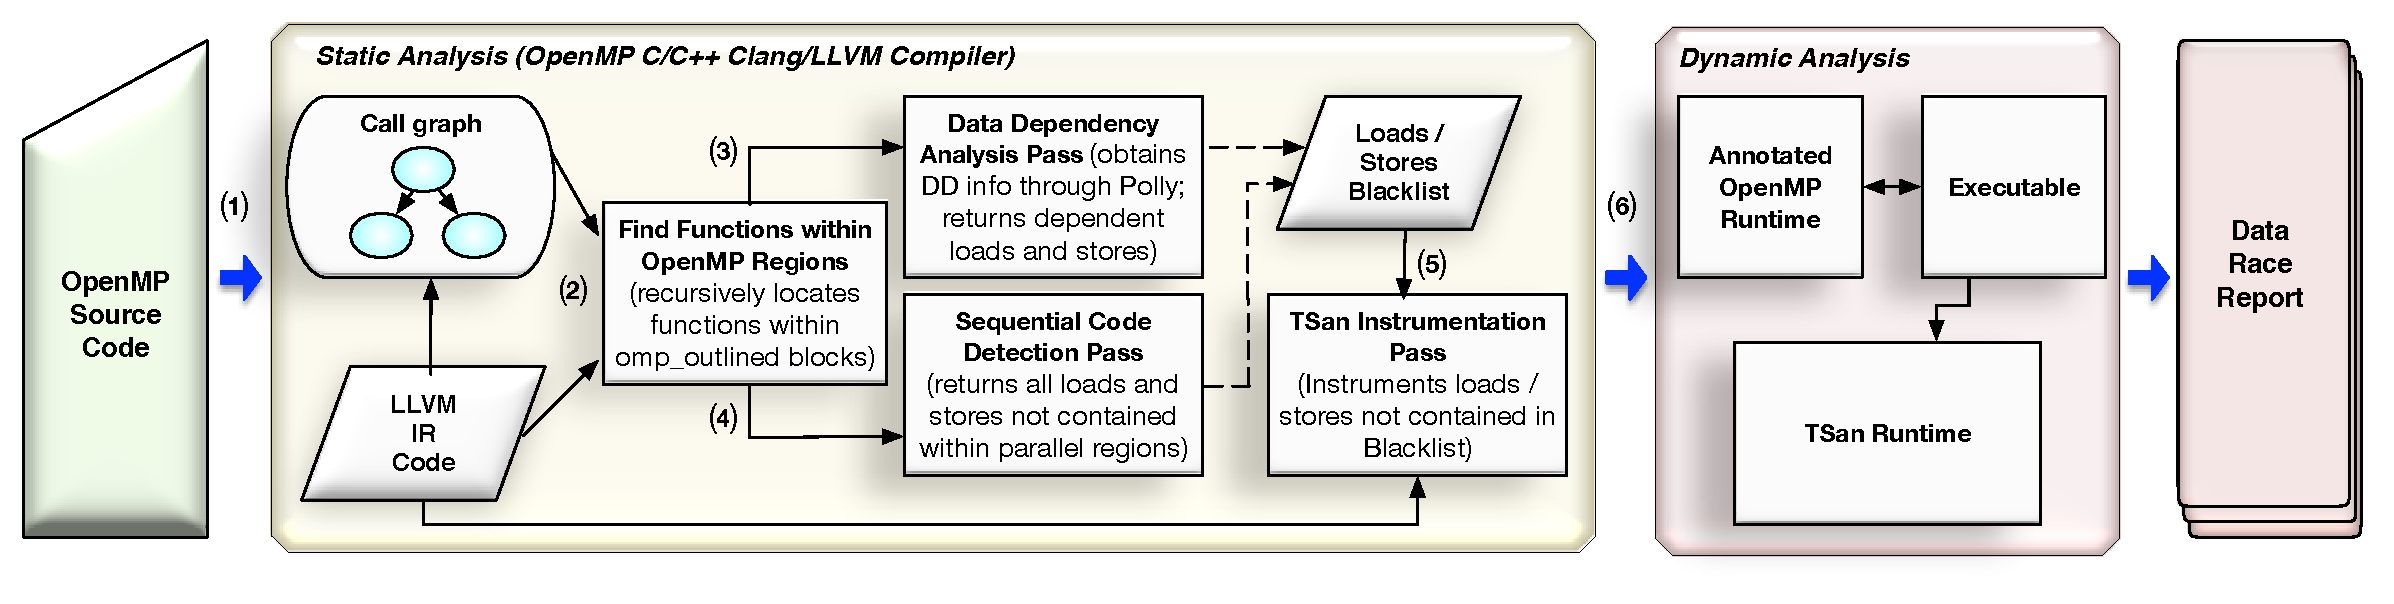
\includegraphics[width=\textwidth]{archerdiagram}
  \vspace{-20pt}
  \caption{\archer tool flow}
  \label{fig:archerdiagram}
  \vspace{-5pt}
\end{figure*}

Figure~\ref{fig:archerdiagram} illustrates how \archer implements our approach
by combining well-layered and modular static- and dynamic-analysis stages.
%
In more detail, our static analysis
passes~\cite{Kennedy:2001:OCM:502981,Muchnick:1998:ACD:286076,polly} help
classify the given OpenMP code regions into two categories: \emph{guaranteed
  race-free} and \emph{potentially racy}.
%
Our dynamic analysis then applies state-of-the-art data-race detection
algorithms~\cite{tsan:2009,Flanagan:2009} to check only the potentially racy
OpenMP regions of code.
%
The static/dynamic analysis combination is central to the scalability ({\em
  while maintaining analysis precision}) of \archer, as evidenced by its
ability to handle real-world examples that existing tools cannot handle with
the same levels of precision and scalability.
%
We implemented \archer using the
LLVM/Clang~\cite{lattner2004llvm} tool infrastructure and the
\tsan dynamic race checker~\cite{tsan}.
%
On the static analysis side, \archer uses Polly~\cite{polly} to perform data
dependency and loop-carried data-dependency analysis (together called {\em
  data dependency analysis} from now on).
%
This results in a {\em Parallel Blacklist}.
%
\archer also extends some of the static verification passes already present in
LLVM.
%
Specifically, these passes build a Call Graph and then traverse it to identify
memory accesses that will not come from within an OpenMP construct (i.e.,
sequential code regions).
%
This results in a {\em Sequential Blacklist}.
%
These blacklists are combined and used to limit the instrumentation in \tsan.
%
On the dynamic analysis side, \archer uses our customized version of \tsan to
detect data races at runtime.
%
To prevent \tsan from being confused by OpenMP runtime internal actions (and
falsely report them as OpenMP-level races), \archer employs \tsan's Annotation
API to highlight these synchronization points within \omp (the OpenMP library
presently associated with \archer in our studies).

We evaluate \archer on a small and large benchmark, respectively the OmpSCR
benchmark suite~\cite{ompscr} (an OpenMP source code collection) and
\amg, a non-trivial application, based on the Hypre library, from
the HPC CORAL benchmark suite~\cite{coral}.
% ; and finally through the HYDRA case study
%
Our evaluation is in terms of the effectiveness, performance, and scalability
of \archer compared to \insp and an unmodified version of \tsan applied to the
same benchmarks.
%
In terms of performance, the experimental results for all benchmarks show that
Archer is between two and ten time faster than \insp.
%
Also, \archer with static analysis support is overall 15\% faster on the
average with respect the only dynamic check performed by the \tsan runtime
with the OpenMP support.
%
In terms of effectiveness \archer (with and without static analysis support)
never misses a race and never reports false positives, while \insp and the
original version of \tsan report a large number of false positives and miss
some of the races.

\vspace{-10pt}
{\footnotesize
\newcommand{\BIBdecl}{\setlength{\itemsep}{0.25 em}}
\bibliographystyle{abbrv}
\bibliography{references}}
\end{document}
